\begin{frame}{Présentation Symfony2}
  Symfony2 c'est :
  \begin{itemize}
  \item Symfony2 (évidemment...)
  \item Twig
  \item Doctrine2
  \item et bien d'autres...
  \end{itemize}
\end{frame}

\begin{frame}{Structure d'un projet Symfony2}
  4 répertoires :
  \begin{description}
    \item[app] configuration, logs, etc.
    \item[src] code source
    \item[vendor] bibliothèques
    \item[web] images, css, etc.
  \end{description}
\end{frame}

\begin{frame}
   \begin{figure}
    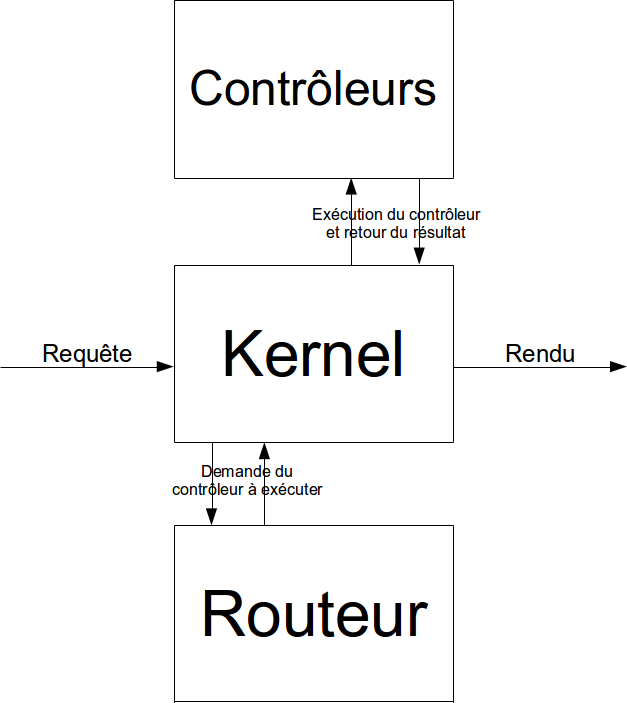
\includegraphics[scale=0.25]{img/fonctionnement.png}
  \end{figure}  
\end{frame}

\begin{frame}[fragile]
  Exemple de code Symfony2 :
  \begin{lstlisting}[language=c++]
     namespace Exemple\ExBundle\Controller;
     use Symfony\Bundle\FrameworkBundle\Controller\Controller;
     use Symfony\Component\HttpFoundation\Response;
     class ExController extends Controller
     {
       public function exempleAction()
       {
         return new Response("Hello world !");
       }
     }
  \end{lstlisting}
\end{frame}

\begin{frame}[fragile]
  Exemple de code Twig :
  \begin{lstlisting}[language=html]
     <div>
     Pseudo : {{ pseudo }} <br />
     Le : {{ last_connect }} <br />
     A : {{ lieu }}
     </div>
  \end{lstlisting}
\end{frame}
